\documentclass[dvipdfmx]{jsarticle}

\usepackage{amsmath,mathtools}
\usepackage{amssymb}
\usepackage{bm}
\usepackage[dvipdfmx]{graphicx}
\usepackage{listings}
\usepackage{xcolor}
\usepackage{indentfirst}
\usepackage{placeins}

\lstset{
    language=Fortran,
    basicstyle=\ttfamily\small,
    keywordstyle=\color{blue},
    commentstyle=\color{green!50!black},
    stringstyle=\color{red},
    numbers=left,
    numberstyle=\tiny,
    stepnumber=1,
    numbersep=10pt,
    frame=single,
    breaklines=true,
    tabsize=4,
    showstringspaces=false
}

\title{計算機ゼミ 課題4}

\author{石川曹太}
\date{\today}

\begin{document}
\maketitle

\section{問題設定}
今回の課題では，一次元拡散方程式を数値的に解き，その結果を解析解と比較することで数値解法の精度を検証する．拡散方程式は熱伝導現象や物質拡散など，時間とともに物理量が空間的に広がっていく現象を表す代表的な偏微分方程式であり，数値解析の基礎として広く用いられている．

今回の課題で対象とする方程式は，以下で与えられる．

\begin{align}
  \frac{\partial u}{\partial t} = \nu \frac{\partial^2 u}{\partial x^2}
\end{align}

ここで，$u(x,t)$は位置$x$，時刻$t$における未知関数であり，熱伝導問題では温度，拡散問題では濃度に対応する．また，$\nu$は拡散係数と呼ばれ，拡散のしやすさを表す定数である．本課題において初期条件は，
\begin{align}
  u(x,0)=
  \begin{cases}
    0 & (x=0)\\
    1 & (otherwise)
  \end{cases}
\end{align}
となる．また，境界条件は左端と右端で異なり，それぞれ
\begin{align}
  u(0,t) = 0 ,\qquad \partial_xu(L,t) = 0
\end{align}
である．一つ目の式はDirichlet境界条件と呼ばれ，境界での未知量そのものを既知値として固定する条件である．一方二つ目の式はNeumann境界条件と呼ばれ，境界における空間微分を指定する条件であり，本課題では右端における流束が存在しないことを意味している．\\

\section{格子点の導入}
偏微分方程式をコンピュータで数値的に解くためには，連続的な空間と時間を有限個の点へ分割する必要がある．そのため，空間方向および時間方向をそれぞれ離散化し，各格子点における未知量を計算する．\\

まず初めに解析領域$0\le x\le L$を$N_x$等分し，空間の刻み幅を
\begin{align}
  \Delta x = \frac{L}{N_x}
\end{align}
と定義する．この時の各格子点の座標は，
\begin{align}
  x_i = i \Delta x \qquad (i = 0,1,\dots,N_x)
\end{align}
で表される．\\

また，時間方向についても一定の時間の刻み幅$\Delta t$を用いて離散化し，以下のように定義する．
\begin{align}
  t^n = n \Delta t \qquad (n = 0,1,2,\dots)
\end{align}
これらの格子点における未知関数は
\begin{align}
  u^n_i = u(x_i,t^n)
\end{align}
と表すことにする．ここで，添え字$i$は空間方向の格子番号，添え字$n$は時間方向の格子番号を表している．\\
このように連続な関数を有限個の格子点上の値で表現することにより，偏微分方程式を代数方程式へ変換し，コンピュータによる数値計算が可能となる．

\section{陽解法}
陽解法とは，現在時刻における未知量のみを用いて次の時刻の未知量を計算する手法である．そのため，一度現在時刻の値が求まれば，行列計算などを行うことなく順次時間発展させることができる．この特徴から計算手順が単純であり，実装が容易であるという利点を持つ．\\

陽解法では式(1)における左辺(時間項)を現在時刻$t^n$と次の時刻の$t^{n+1}$の値を用いた前進差分によって近似する．
\begin{align}
  \frac{\partial u}{\partial t} \approx \frac{u_i^{n+1}-u_i^n}{\Delta t}
\end{align}\\

一方，式(1)における右辺(空間方向の二階微分)は中央差分によって以下のように近似可能である．
\begin{align}
  \frac{\partial^2 u}{\partial x^2} \approx \frac{u_{i+1}^n - 2 u_i^n + u_{i-1}^n}{\Delta x^2}
\end{align}\\

ここで，右辺の空間微分は全て現在時刻$n$における値で評価していることに注意する．このように現在時刻の情報のみを利用することが，陽解法と呼ばれる理由である．
これらを支配方程式(1)に代入すると，
\begin{align}
  \frac{u_i^{n+1}-u_i^n}{\Delta t} = \nu \frac{u_{i+1}^n - 2 u_i^n + u_{i-1}^n}{\Delta x^2}
\end{align}
を得る．ここで両辺に$\Delta t$をかけて未知量$u_i^{n+1}$について整理すると，以下の式を得る．
\begin{align}
  u_i^{n+1} = u_i^n + r(u_{i+1}^n - 2u_i^n + u_{i-1}^n) , \qquad r = \nu \frac{\Delta t}{\Delta x^2}
\end{align}
ここで$r$は離散化パラメータである．この式(11)が本課題でFortranプログラムに実装した陽解法の更新式である．実際のプログラムでは．この式を内部格子点$i=1,\dots,N_x-1$に対して繰り返し適用することで，時刻$t=0$から最終時刻$T_{max}$まで数値解を逐次計算した．\\

陽解法は計算手順が単純で実装も容易である一方，時間刻み幅を自由に設定できるわけではない．時間刻み幅が大きすぎると，数値誤差が時間とともに増幅し，数値解が発散する可能背うがある．そこで，一次元拡散方程式に対する陽解法では，Von \, Neumann安定性解析より，離散化パラメータ$r$は
\begin{align}
  r = \nu \frac{\Delta t}{\Delta x^2} \le 0.5
\end{align}
を満たさなければならないことが知られている．そのため，本課題で作成したプログラムでは，計算開始時に離散化パラメータを計算し，この条件を満たしているか確認した．条件を満たさない場合には数値計算を実行せず，プログラムを終了するように実装している．


\section{陰解法}
陰解法では，時間方向の差分近似は陽解法と同様に前進差分を用いるが，空間方向の二階微分を次の時刻$n+1$における未知量で評価する点が陽解法との大きな違いである．\\

時間方向の微分は陽解法と同様に以下のように近似する．
\begin{align}
  \frac{\partial u}{\partial t} \approx \frac{u_i^{n+1}-u_i^n}{\Delta t}
\end{align}\\

一方，空間方向の二階微分に関しては，現在時刻ではなく次の時刻の値を用いて以下のように近似する．
\begin{align}
  \frac{\partial^2 u}{\partial x^2} \approx \frac{u_{i+1}^{n+1} - 2 u_i^{n+1} + u_{i-1}^{n+1}}{\Delta x^2}
\end{align}\\

これらの式を拡散方程式(1)に代入すると，
\begin{align}
  \frac{u_i^{n+1}-u_i^n}{\Delta t} = \nu \frac{u_{i+1}^{n+1} - 2 u_i^{n+1} + u_{i-1}^{n+1}}{\Delta x^2}
\end{align}
を得る．ここで両辺に$\Delta t$をかけて$u_i^n$について整理すると，以下の式を得る．
\begin{align}
  -ru_{i-1}^{n+1} + (1+2r)u_i^{n+1} -ru_{i+1}^{n+1} = u_i^n
\end{align}
これが陰解法における基本的な差分方程式である．\\

式(16)を見ると，ある格子点$i$の未知量だけではなく$u_{i-1}^{n+1}，u_i^{n+1}，u_{i+1}^{n+1}$の3つが同時に含まれていることが分かる．つまり，ある1点だけを計算することができず，すべての内部格子点を同時に求めなければならない．そこで，各格子点の式をまとめて一つの連立一次方程式として表現する．
内部節点のみを未知数として並べたベクトルを

\[
\mathbf{u}^{\,n+1}
=
\begin{bmatrix}
u_1^{n+1}\\
u_2^{n+1}\\
\vdots\\
u_{N_x-1}^{n+1}
\end{bmatrix}
\]

と定義する．同様に，現在時刻における未知量ベクトルを

\[
\mathbf{u}^{\,n}
=
\begin{bmatrix}
u_1^{n}\\
u_2^{n}\\
\vdots\\
u_{N_x-1}^{n}
\end{bmatrix}
\]

と定義する．式(16)をすべての内部節点について書き並べると，

\[
\begin{aligned}
(1+2r)u_1^{n+1}-ru_2^{n+1}
&=u_1^n,\\
-r u_1^{n+1}
+(1+2r)u_2^{n+1}
-r u_3^{n+1}
&=u_2^n,\\
-r u_2^{n+1}
+(1+2r)u_3^{n+1}
-r u_4^{n+1}
&=u_3^n,\\
&\ \vdots\\
-r u_{N_x-2}^{n+1}
+(1+r)u_{N_x-1}^{n+1}
&=u_{N_x-1}^n.
\end{aligned}
\]

これらの連立方程式を行列形式で表すと，

\[
\begin{bmatrix}
1+2r & -r    & 0     & \cdots & 0\\
-r   & 1+2r  & -r    & \ddots & \vdots\\
0    & -r    & 1+2r  & \ddots & 0\\
\vdots & \ddots & \ddots & \ddots & -r\\
0 & \cdots & 0 & -r & 1+r
\end{bmatrix}
\begin{bmatrix}
u_1^{n+1}\\
u_2^{n+1}\\
\vdots\\
u_{N_x-2}^{n+1}\\
u_{N_x-1}^{n+1}
\end{bmatrix}
=
\begin{bmatrix}
u_1^{n}\\
u_2^{n}\\
\vdots\\
u_{N_x-2}^{n}\\
u_{N_x-1}^{n}
\end{bmatrix}
\tag{28}
\]

となる．本課題におけるプログラムでは，この係数行列を$\boldsymbol{A}$とし，課題3のモジュールを用いて逆行列を計算することで，現在の時刻におけるすべての内部点から次の時刻におけるすべての内部点における数値を求める式を以下のように得る．
\begin{align}
  \boldsymbol{u}^{n+1} = \boldsymbol{A}^{-1} \boldsymbol{u}^n
\end{align}\\

ここで用いた陰解法という手法は，各時間ステップで連立一次方程式を解く必要があるため計算量は増加するものの，一次元拡散方程式に対しては無条件安定であり，陽解法のような厳しい安定条件を受けない．そのため，大きな時間刻み幅を用いても安定した計算を行うことができるという利点を持っている．

\subsection{境界条件の反映}

差分法では内部格子点だけでなく，境界点における未知量も適切に扱う必要がある。本課題では，左端ではDirichlet境界条件，右端ではNeumann境界条件を与えているため，それぞれ異なる方法で差分式へ反映した．まず，左端境界では

\begin{align}
  u(0,t)=0
\end{align}

が与えられている．これはDirichlet境界条件と呼ばれ，境界における未知量そのものが既知であることを意味する．そのため，差分近似を行う必要はなく，常に

\begin{align}
  u_0^n=0
\end{align}

と与えればよい．実際のプログラムにおいても，各時間ステップごとに

\begin{align}
  u_0^{\,n+1}=0
\end{align}

を代入することで境界条件を満たしている．一方，右端では

\begin{align}
  \frac{\partial u}{\partial x}(L,t)=0
\end{align}

が与えられている．これはNeumann境界条件であり，境界における空間微分（流束）が零であることを意味する．この一階微分を後退差分で近似すると，

\begin{align}
  \frac{\partial u}{\partial x}
  \approx
  \frac{u_{N_x}-u_{N_x-1}}
  {\Delta x}
\end{align}

となる．境界条件より

\begin{align}
  \frac{u_{N_x}-u_{N_x-1}}
  {\Delta x}
  =
  0
\end{align}

であるから，

\begin{align}
  u_{N_x}
  =
  u_{N_x-1}
\end{align}

が得られる．したがって，右端境界では境界点の値を一つ内側の格子点と等しく設定することによって，Neumann境界条件を満足させることができる．陽解法では，各時間ステップで内部格子点の更新を行った後，

\begin{align}
  u_{N_x}^{\,n+1}
  =
  u_{N_x-1}^{\,n+1}
\end{align}

と代入することで境界条件を反映した．

一方，陰解法では，この境界条件を係数行列の構築時にあらかじめ組み込んでいる．陰解法では最後の内部節点に対する差分式は

\begin{align}
  -r u_{N_x-2}^{\,n+1}
  +
  (1+2r)u_{N_x-1}^{\,n+1}
  -
  r u_{N_x}^{\,n+1}
  =
  u_{N_x-1}^{\,n}
\end{align}

となるが，ここでNeumann境界条件

\begin{align}
  u_{N_x}^{\,n+1}
  =
  u_{N_x-1}^{\,n+1}
\end{align}

を代入すると，

\begin{align}
  -r u_{N_x-2}^{\,n+1}
  +
  (1+r)u_{N_x-1}^{\,n+1}
  =
  u_{N_x-1}^{\,n}
\end{align}

となる．この結果，係数行列の最終行は

\begin{align}
  \begin{bmatrix}
  \cdots
  &
  -r
  &
  1+r
  \end{bmatrix}
\end{align}

となり，本課題で作成したFortranプログラム中の係数行列

\begin{align}
  A(N_x-1,N_x-2)=-r,\qquad
  A(N_x-1,N_x-1)=1+r
\end{align}

が得られる．\\

以上より，左端のDirichlet境界条件は未知量を直接固定することで，右端のNeumann境界条件は差分近似を用いて係数行列および境界点の値へ反映することで，両境界条件を数値計算に組み込んだ．

\section{解析解}

数値解の精度を評価するため，拡散方程式の解析解を導出する．

対象とする支配方程式は

\begin{align}
\frac{\partial u}{\partial t}
=
\nu
\frac{\partial^2u}{\partial x^2}
\end{align}

である．境界条件は

\begin{align}
u(0,t)=0
\end{align}

および

\begin{align}
\frac{\partial u}{\partial x}(L,t)=0
\end{align}

であり，初期条件は

\begin{align}
u(x,0)=1
\end{align}

とする．まず，変数分離法を用いて

\begin{align}
u(x,t)=X(x)T(t)
\end{align}

と仮定する．これを支配方程式へ代入すると，

\begin{align}
X(x)\frac{dT}{dt}
=
\nu
T(t)\frac{d^2X}{dx^2}
\end{align}

となる.両辺を $\nu X(x)T(t)$ で割ると，

\begin{align}
\frac{1}{\nu T}
\frac{dT}{dt}
=
\frac{1}{X}
\frac{d^2X}{dx^2}
\end{align}

を得る．左辺は時間のみ，右辺は空間のみの関数であるため，両辺は同じ定数に等しくなる．ここで分離定数を $-\lambda$ とおくと，

\begin{align}
\frac{1}{\nu T}
\frac{dT}{dt}
=
\frac{1}{X}
\frac{d^2X}{dx^2}
=
-\lambda
\end{align}

となる．したがって，時間方向と空間方向の微分方程式は

\begin{align}
\frac{dT}{dt}
+\nu\lambda T
=
0
\end{align}

および

\begin{align}
\frac{d^2X}{dx^2}
+\lambda X
=
0
\end{align}

となる．空間方向の一般解は

\begin{align}
X(x)
=
C_1\cos(\sqrt{\lambda}x)
+
C_2\sin(\sqrt{\lambda}x)
\end{align}

である．左端境界条件

\begin{align}
X(0)=0
\end{align}

より

\begin{align}
C_1=0
\end{align}

となるので，

\begin{align}
X(x)
=
C_2
\sin(\sqrt{\lambda}x)
\end{align}

となる．次に右端境界条件

\begin{align}
\frac{dX}{dx}(L)=0
\end{align}

を適用する．空間微分は

\begin{align}
\frac{dX}{dx}
=
C_2\sqrt{\lambda}
\cos(\sqrt{\lambda}x)
\end{align}

となるので，

\begin{align}
\cos(\sqrt{\lambda}L)=0
\end{align}

が得られる．余弦関数が零となる条件より，

\begin{align}
\sqrt{\lambda}L
=
\frac{(2n+1)\pi}{2},
\qquad
n=0,1,2,\cdots
\end{align}

である．したがって，

\begin{align}
\lambda
=
\left(
\frac{(2n+1)\pi}{2L}
\right)^2
\end{align}

となる．ここでコード中で用いた固有値

\begin{align}
B_n
=
\frac{(2n+1)\pi}{2L}
\end{align}

を導入すると，

\begin{align}
\lambda
=
B_n^2
\end{align}

と表すことができる．時間方向の微分方程式

\begin{align}
\frac{dT}{dt}
+\nu B_n^2T
=
0
\end{align}

を解くと，

\begin{align}
T(t)
=
\exp
\left(
-\nu B_n^2t
\right)
\end{align}

となる．したがって，各固有モードの解は

\begin{align}
u_n(x,t)
=
A_n
\sin(B_nx)
\exp(-\nu B_n^2t)
\end{align}

となる．重ね合わせの原理より，全体の解は

\begin{align}
u(x,t)
=
\sum_{n=0}^{\infty}
A_n
\sin(B_nx)
\exp(-\nu B_n^2t)
\end{align}

となる．初期条件

\begin{align}
u(x,0)=1
\end{align}

を代入すると，

\begin{align}
1
=
\sum_{n=0}^{\infty}
A_n
\sin(B_nx)
\end{align}

となる．両辺に $\sin(B_mx)$ を掛けて $0$ から $L$ まで積分し，三角関数の直交性を利用すると，

\begin{align}
A_n
=
\frac{2}{L}
\int_0^L
\sin(B_nx)\,dx
\end{align}

となる．積分を実行すると，

\begin{align}
A_n
=
\frac{4}{(2n+1)\pi}
\end{align}

を得る．以上より，本課題で用いた解析解は

\begin{align}
u(x,t)
=
\sum_{n=0}^{\infty}
\frac{4}{(2n+1)\pi}
\sin(B_nx)
\exp(-\nu B_n^2t)
\end{align}

ただし，

\begin{align}
B_n
=
\frac{(2n+1)\pi}{2L}
\end{align}

である．実際のプログラムでは無限級数を有限項で打ち切り，

\begin{align}
N_{\mathrm{term}}=100
\end{align}

として100項まで計算を行った．\\


\section{コード}
これらの計算を実装した陽解法，陰解法のコードを以下に示す．\\

\lstinputlisting[language = Fortran, caption={陽解法プログラム}, label = {lst:code1}]{../youkaihou/youkaihou.f90}

\lstinputlisting[language = Fortran, caption={陰解法プログラム}, label = {lst:code2}]{../inkaihou/inkaihou.f90}


\section{実行結果}
作成したコードの実行結果を以下に示す．本課題では，メインプログラムはFortranで実装しており，離散化パラメータと最大誤差を表示するようになっている．離散化された各格子点における数値解はcsvファイルとして出力し，そのデータの図示には，Pythonを使用している．\\

例として，具体的なパラメータを以下のように仮定して実行した結果を図として示す．\\
\begin{align*}
  L = 1.0, \qquad \nu = 1.0, \qquad N_x = 50, \qquad \Delta t = 0.0001, \qquad T_{max} = 0.1
\end{align*}

\begin{figure}[ht]
  \centering
  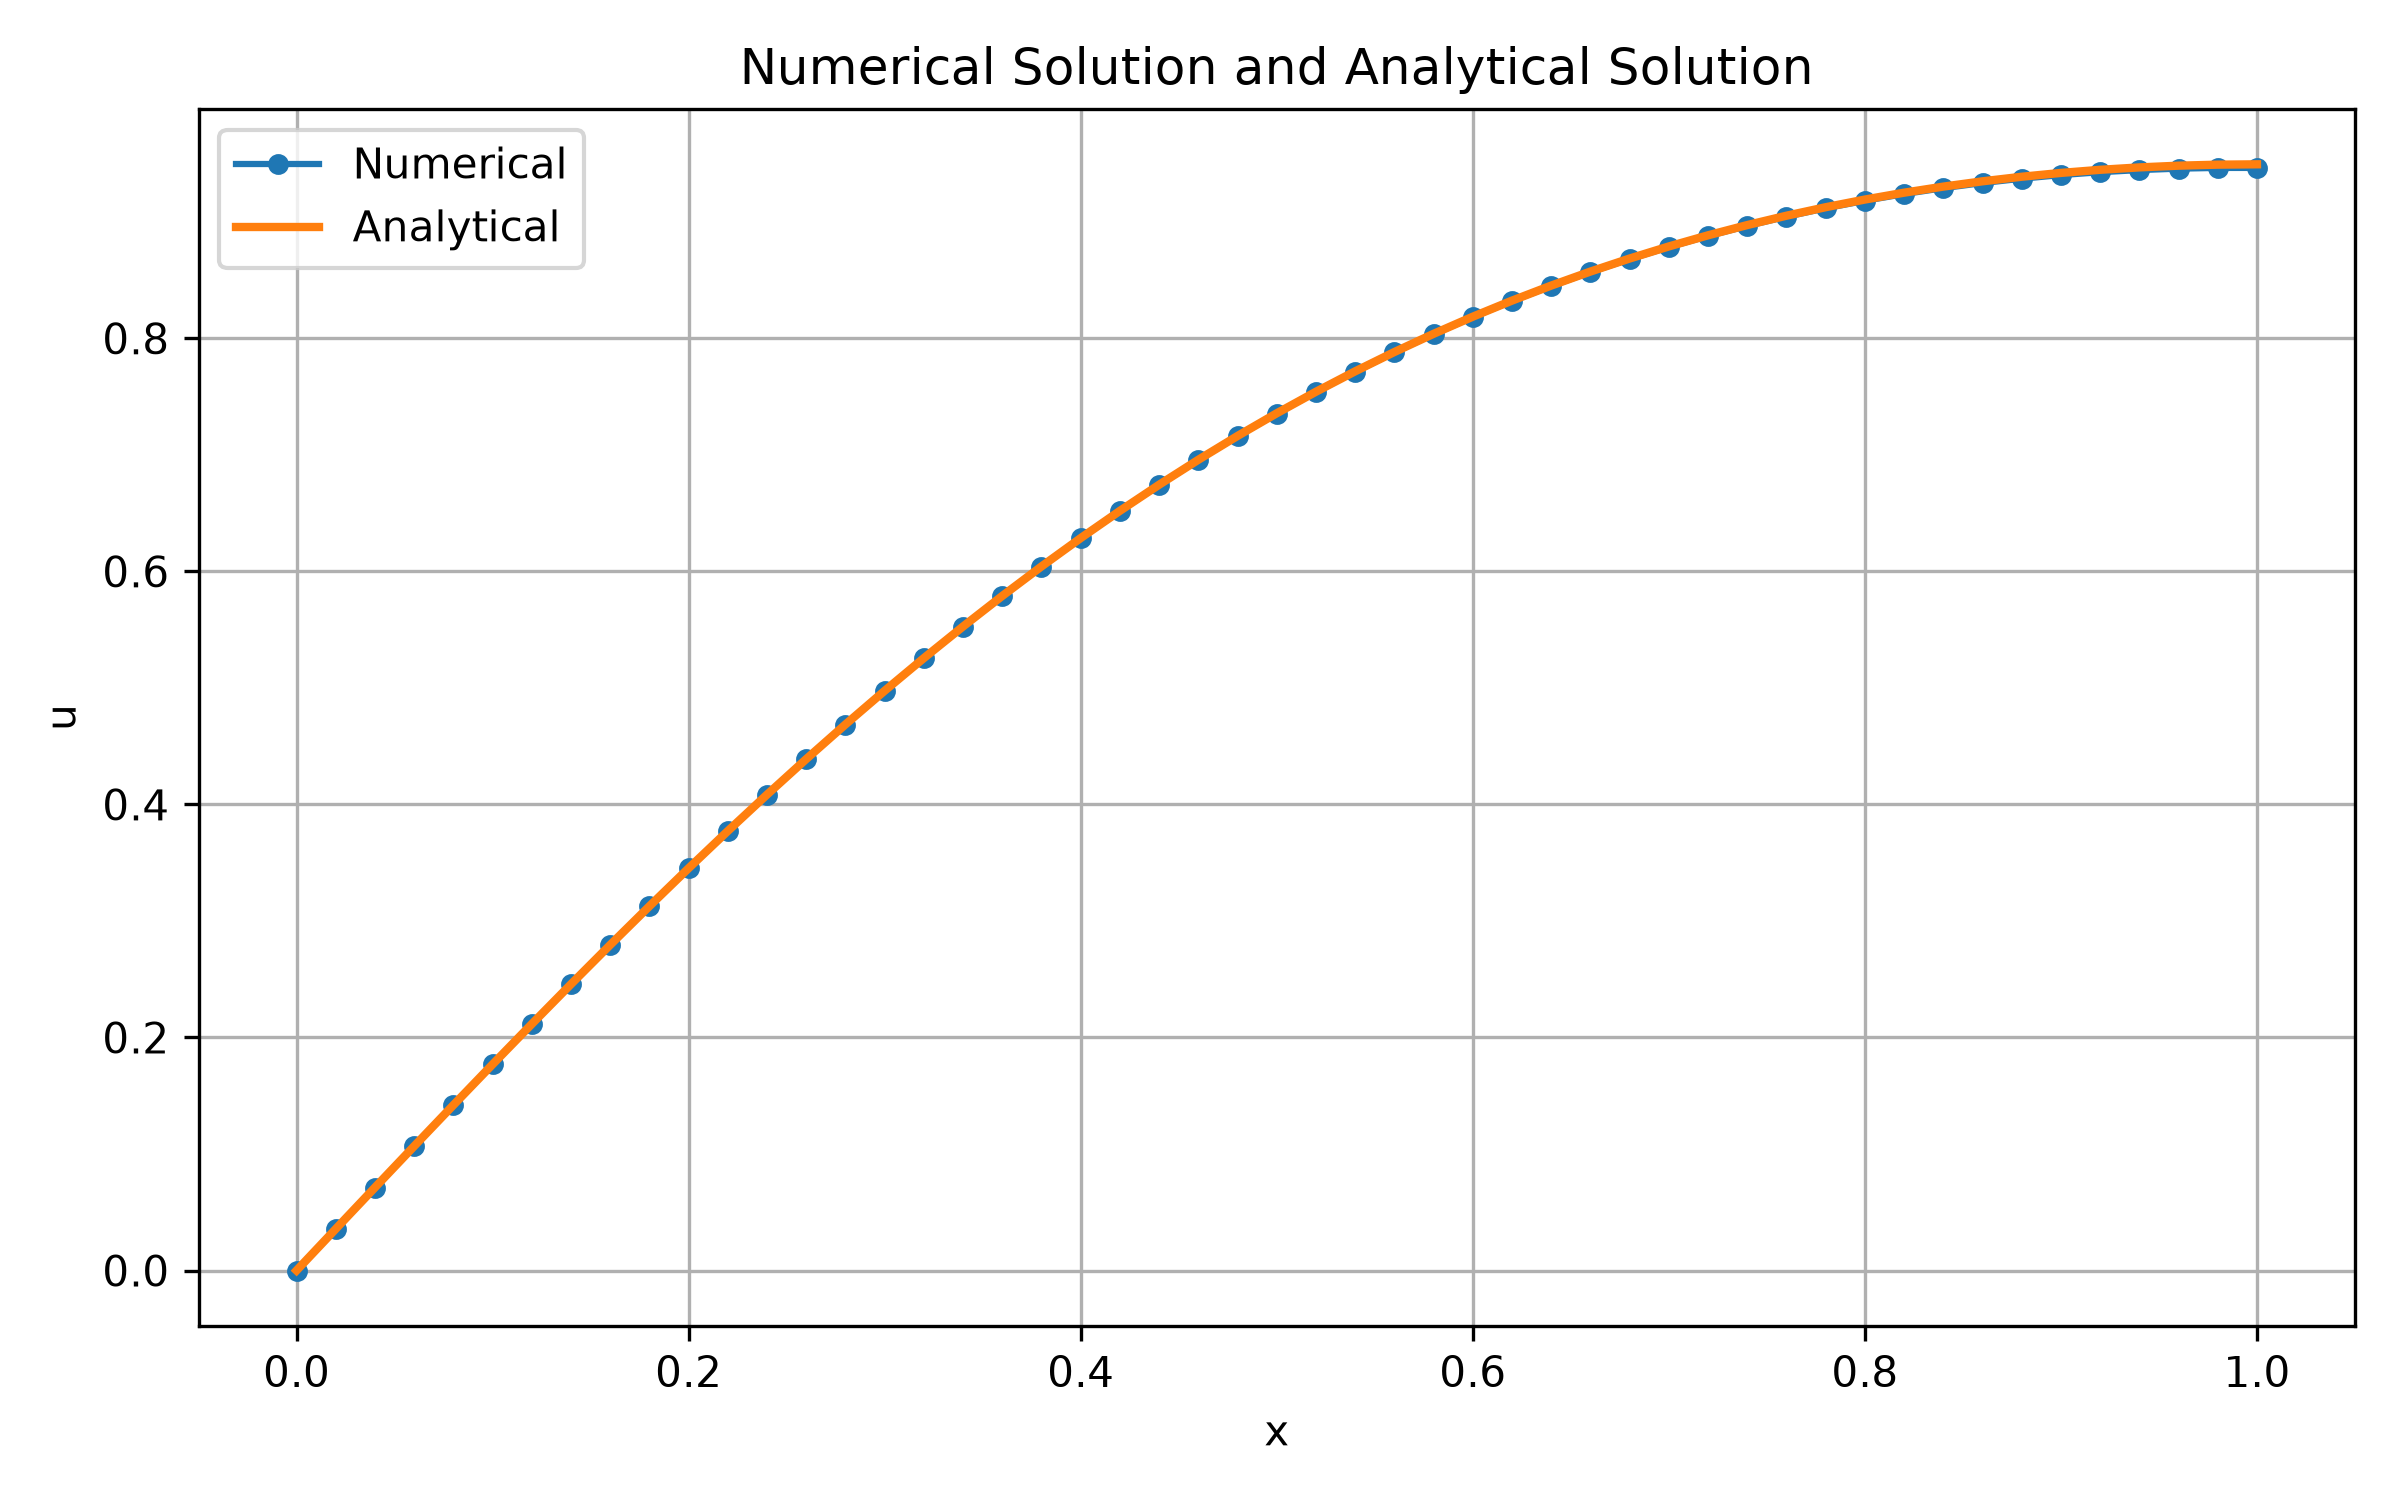
\includegraphics[width=0.8\linewidth]{../youkaihou/youkaihou.png}
  \caption{陽解法の実行結果(数値解と解析解)}
  \label{fig:youkaihouresult}
\end{figure}

\begin{figure}[ht]
  \centering
  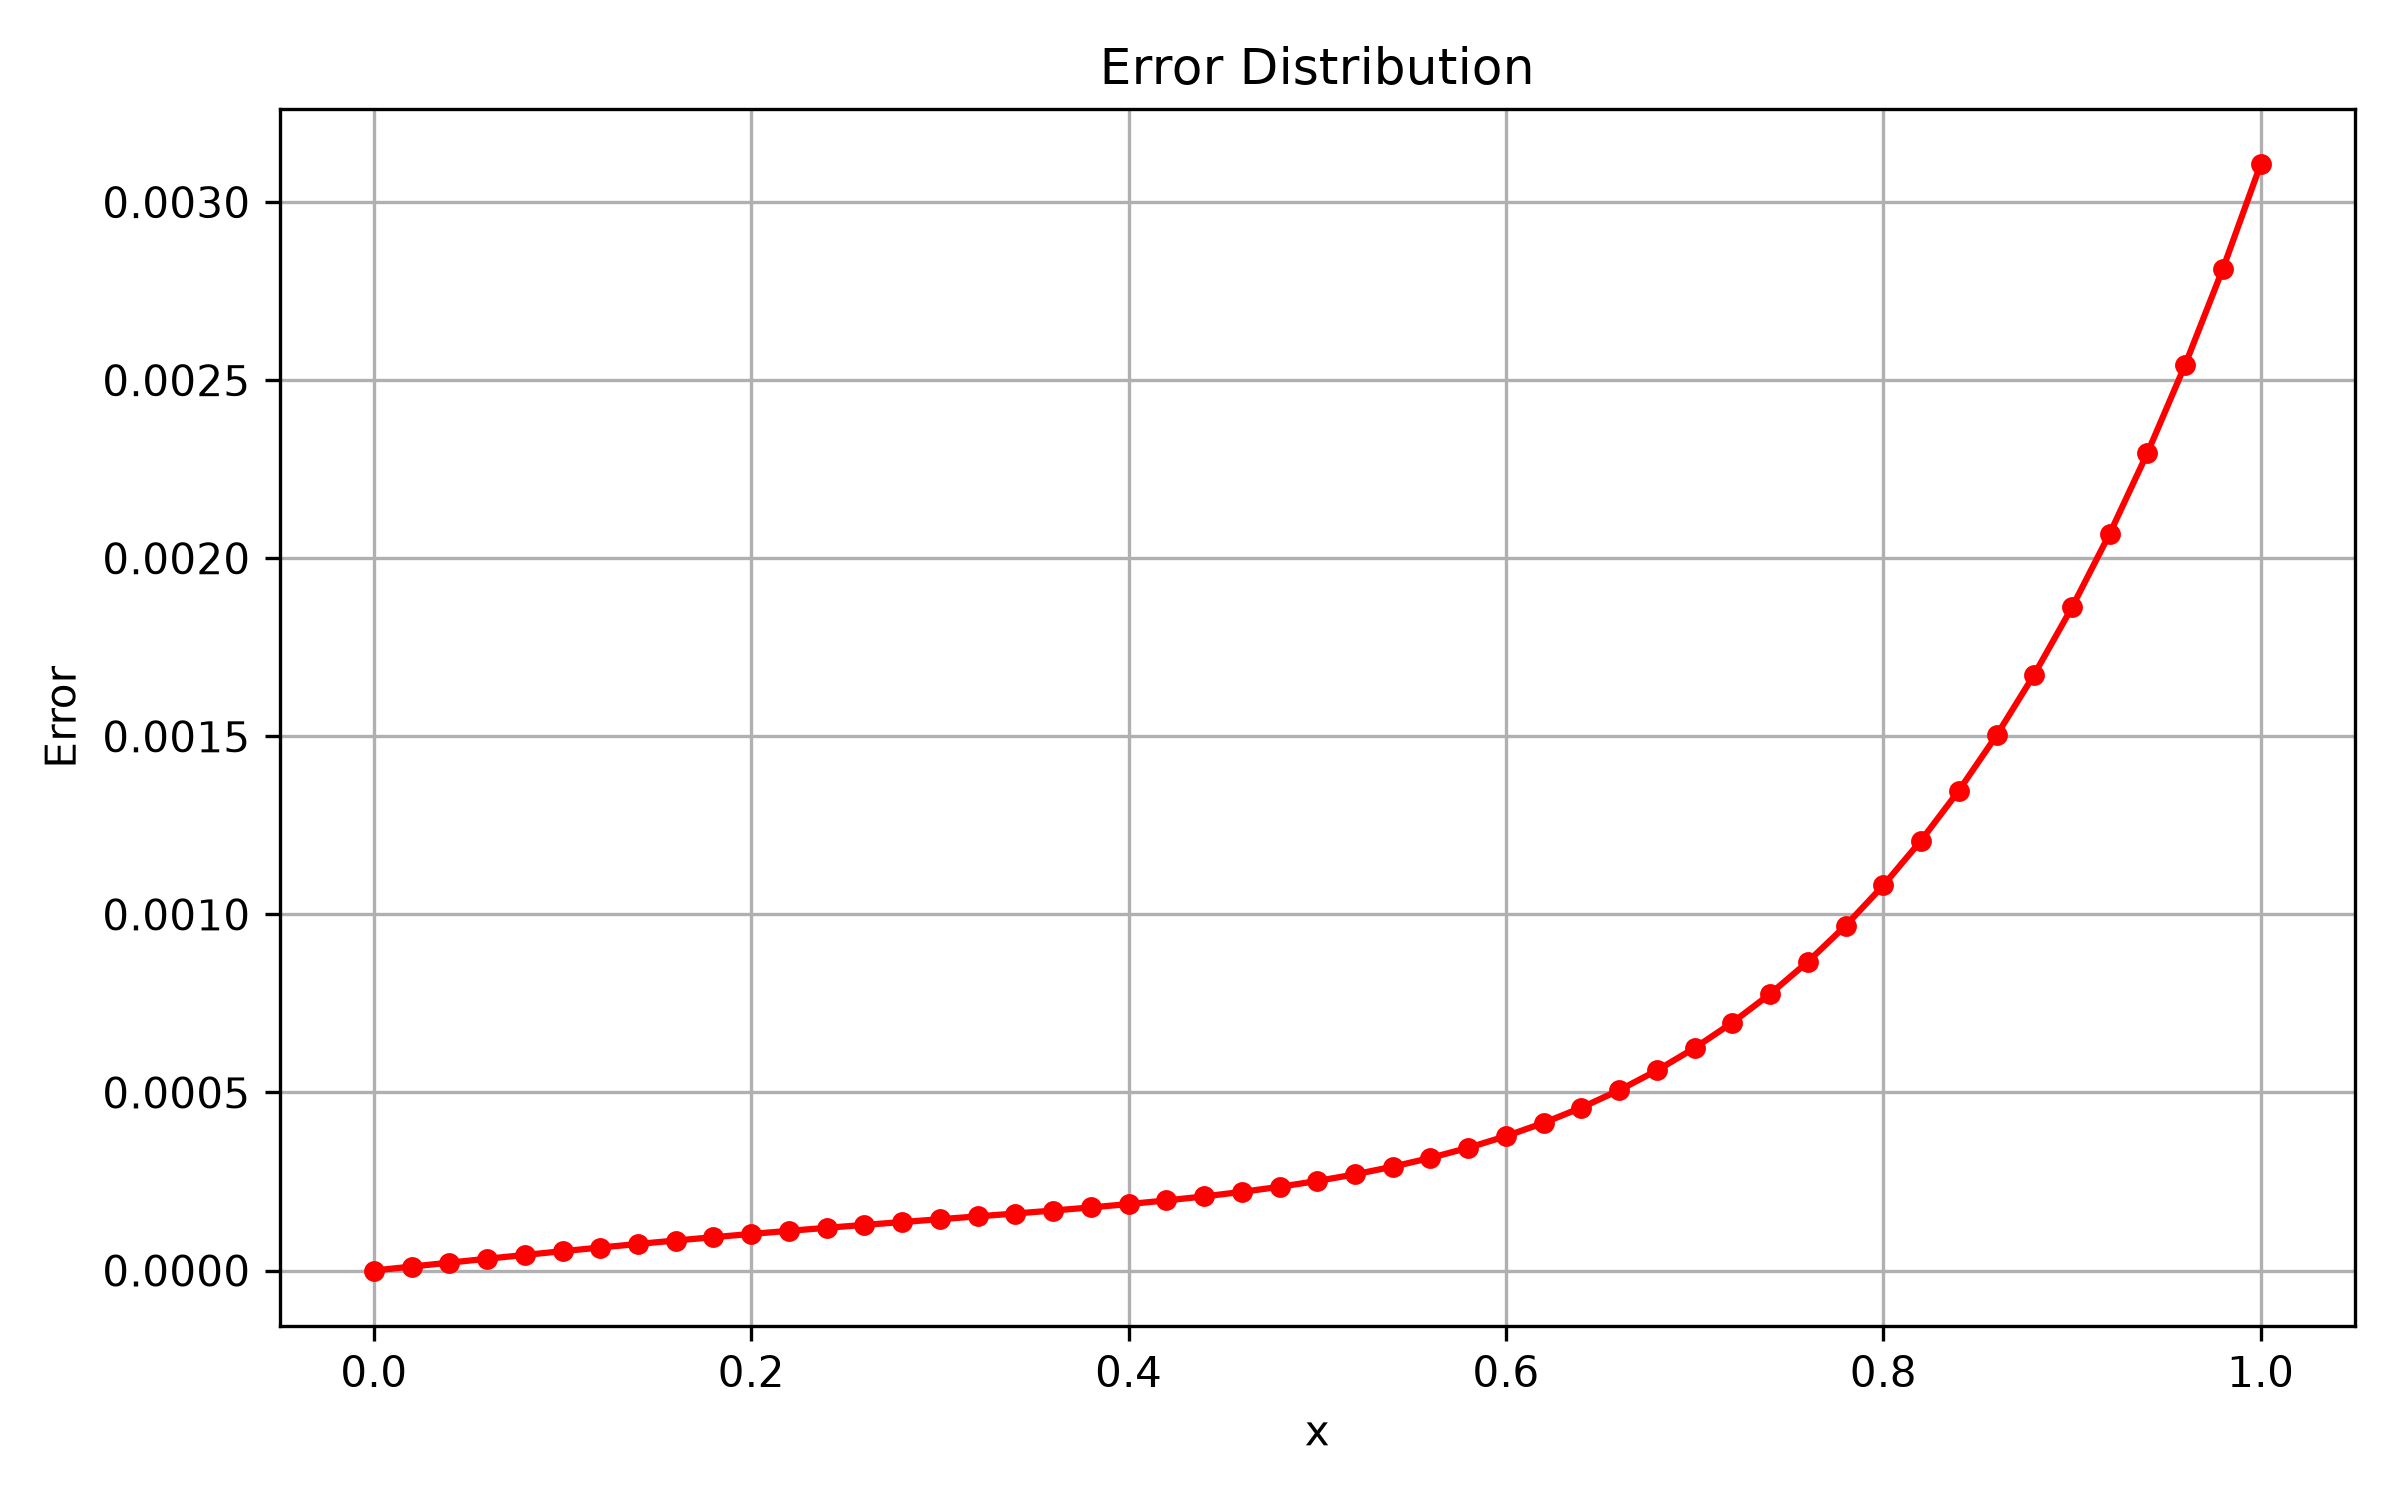
\includegraphics[width=0.8\linewidth]{../youkaihou/erroryou.png}
  \caption{陽解法の実行結果(誤差)}
  \label{fig:youkaihouerror}
\end{figure}

\begin{figure}[ht]
  \centering
  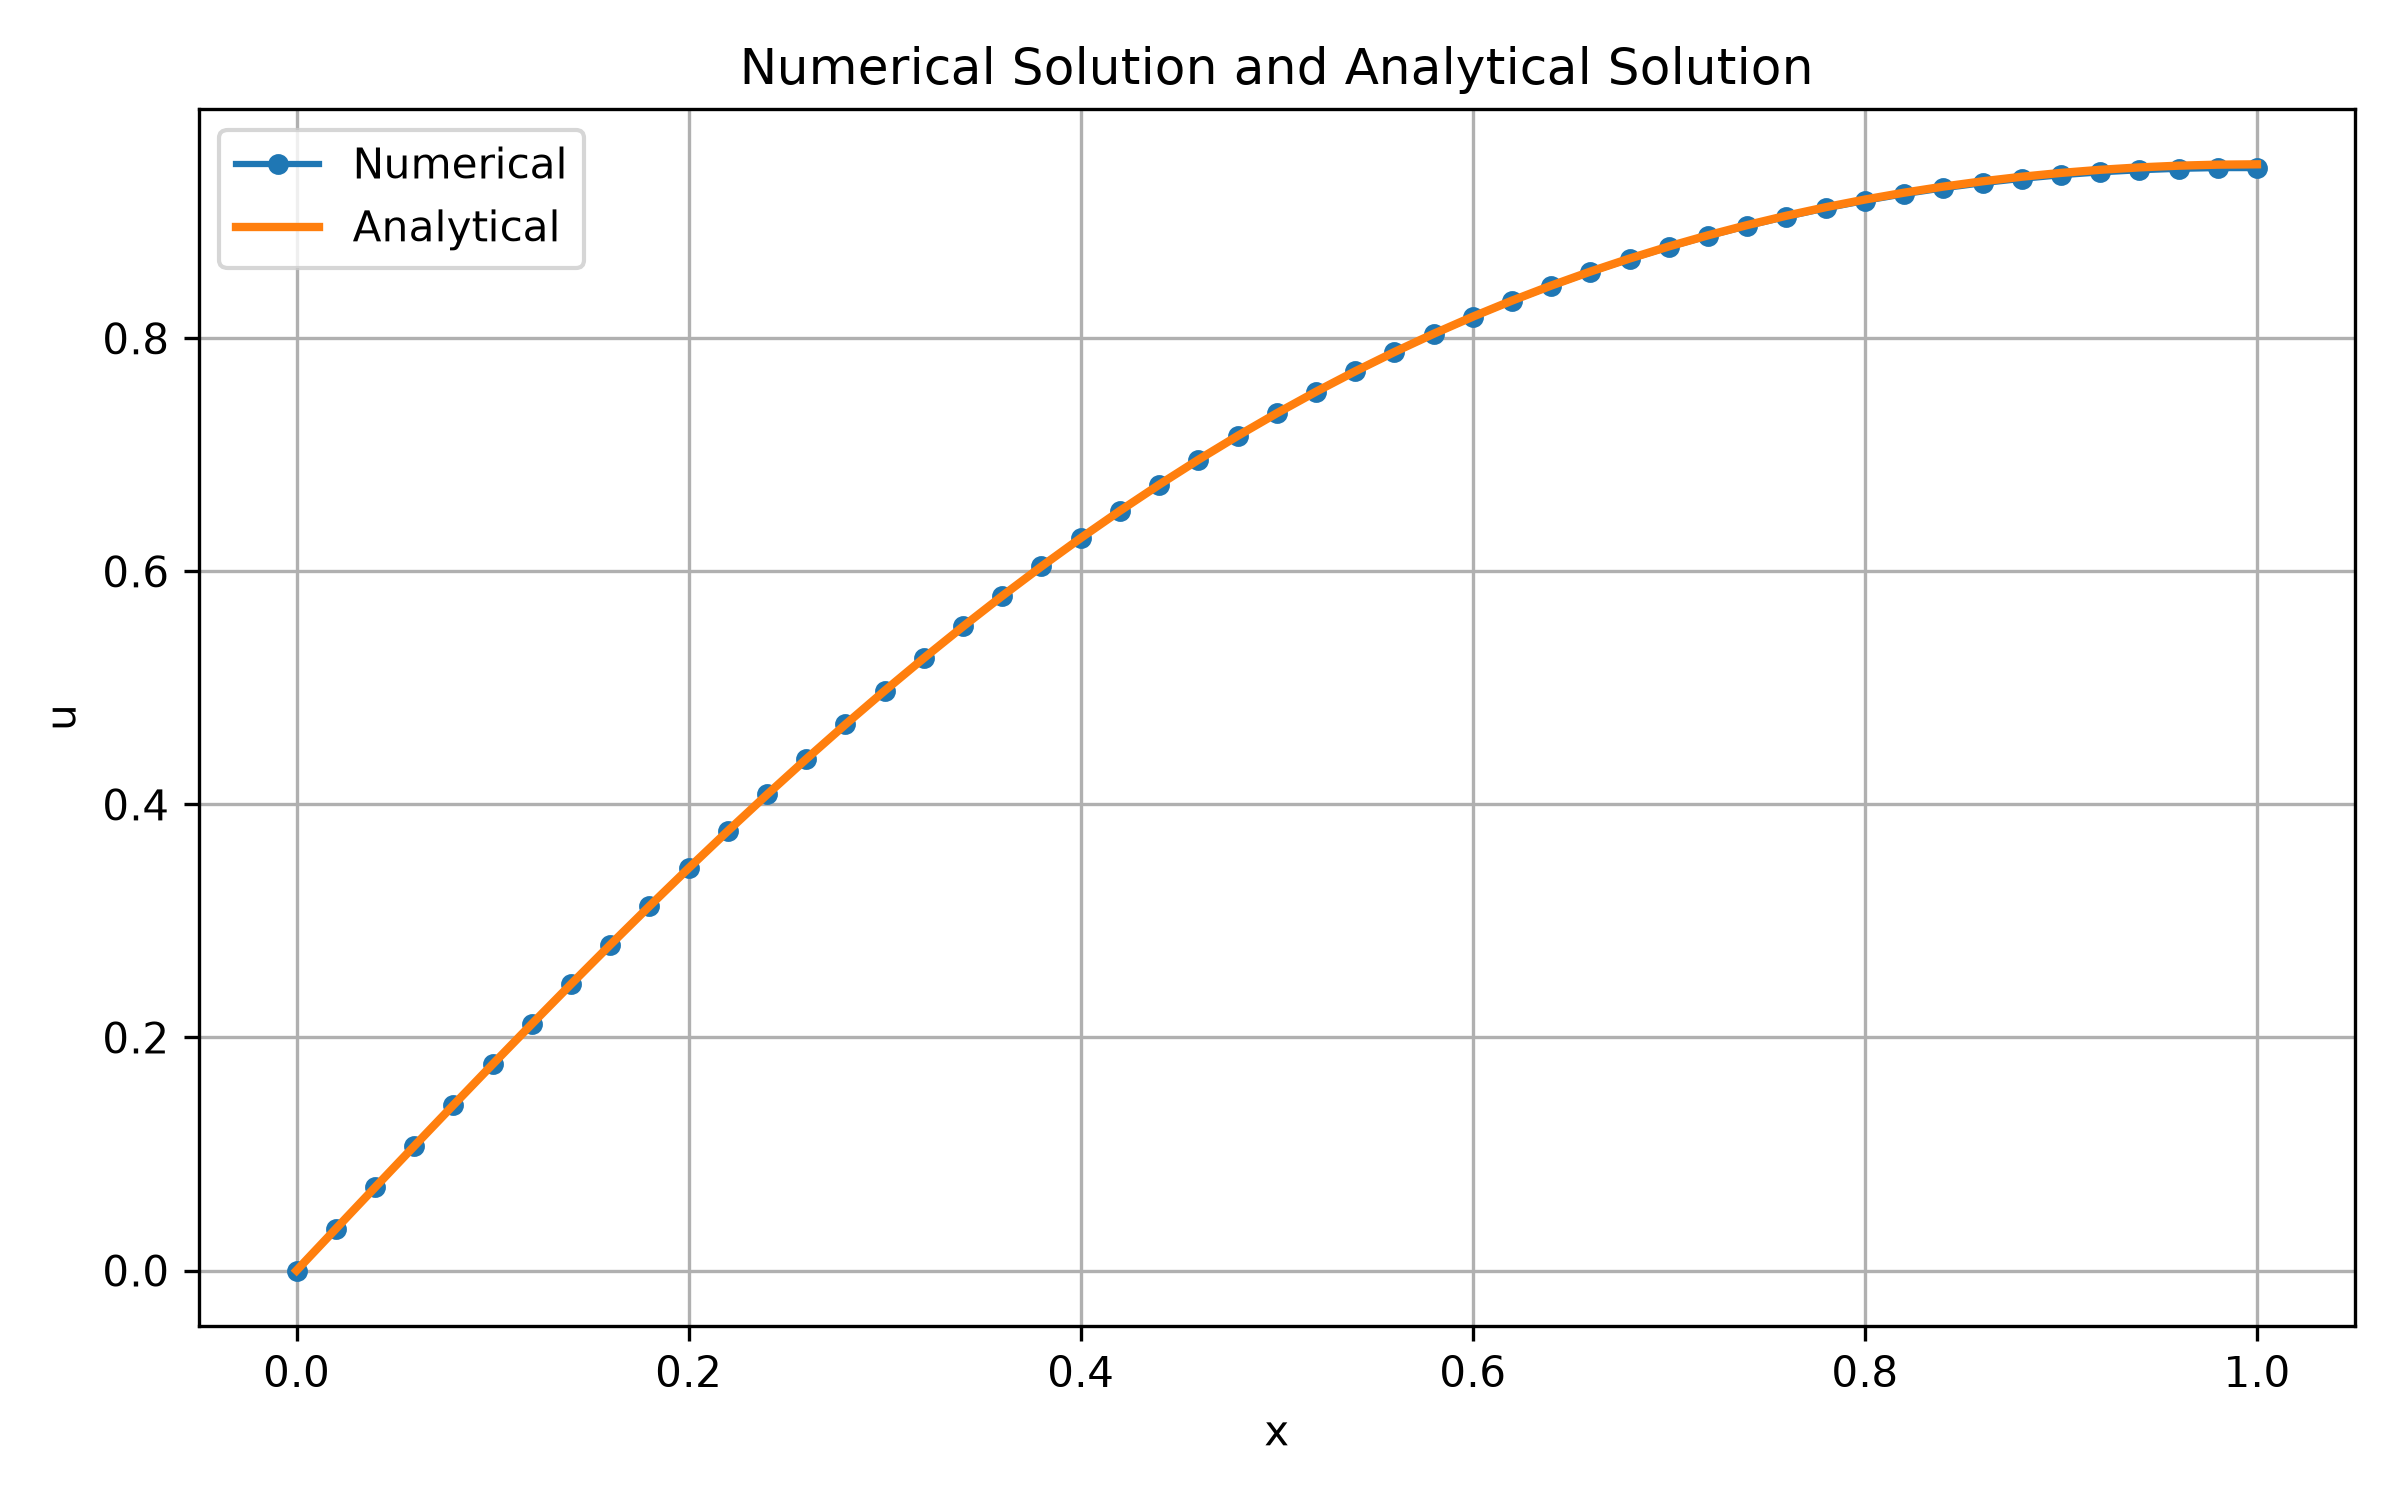
\includegraphics[width=0.8\linewidth]{../inkaihou/inkaihou.png}
  \caption{陰解法の実行結果(数値解と解析解)}
  \label{fig:inkaihouresult}
\end{figure}

\begin{figure}[ht]
  \centering
  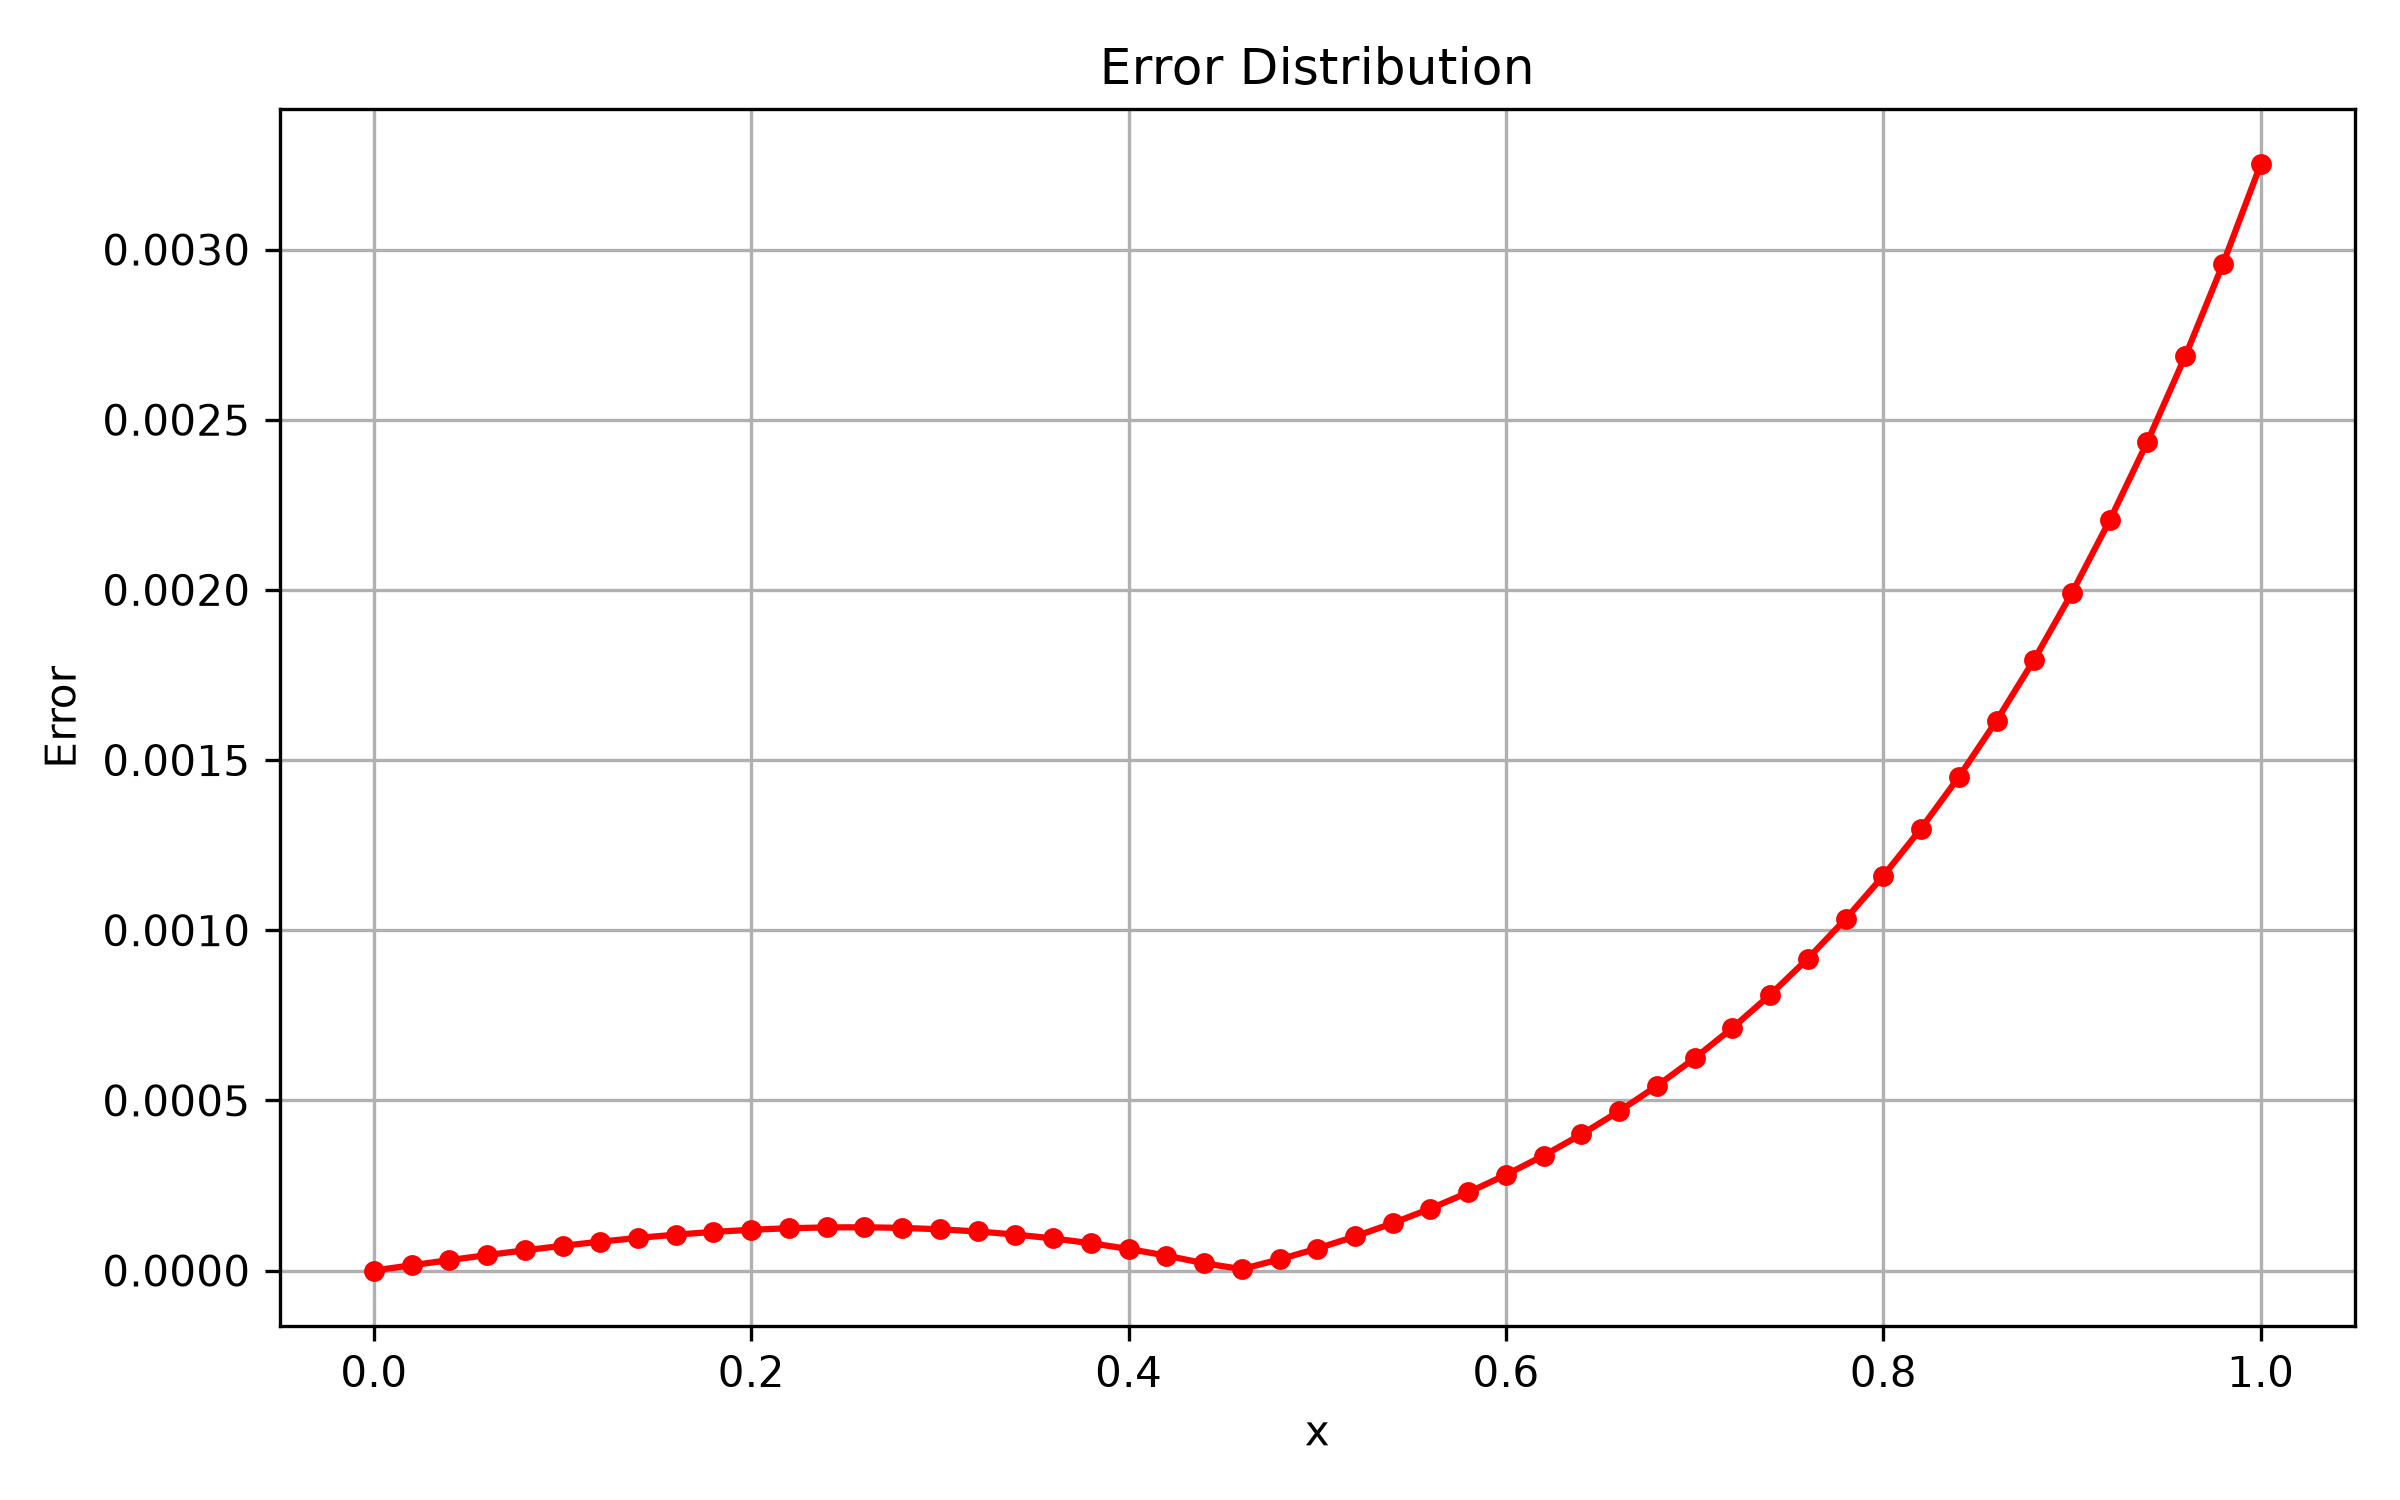
\includegraphics[width=0.8\linewidth]{../inkaihou/errorin.png}
  \caption{陰解法の実行結果(誤差)}
  \label{fig:inkaihouerror}
\end{figure}

\FloatBarrier

ここで，陽解法における最大誤差は約$3.106\times 10^{-3}$，陰解法における最大誤差は約$3.250\times 10^{-3}$であった．


\section{考察}

図1および図3より，陽解法，陰解法ともに数値解は解析解とほぼ重なっており，両手法とも一次元拡散方程式を適切に解くことができていることが確認できた。実際にグラフを比較しても，両者を見分けることが難しいほど一致しており，今回作成したプログラムが正しく実装できていることが分かる。また，誤差分布を示した図2および図4からも，全体として誤差は非常に小さい値に抑えられており，数値計算として十分な精度が得られていると考えられる。

最大誤差を比較すると，陽解法では約 $3.106\times10^{-3}$，陰解法では約 $3.250\times10^{-3}$ となり，陰解法の方がわずかに誤差が大きい結果となった。しかし，その差は約 $1.4\times10^{-4}$ 程度であり，非常に小さい値である。そのため，今回設定した計算条件では，どちらの手法を用いても解析解を十分な精度で再現できていると考えられる。

ここで，図2および図4を見ると，誤差は区間全体で一定ではなく，右端である $x=L$ に近づくにつれて大きくなっていることが分かる。この原因として，右端ではNeumann境界条件

\[
\frac{\partial u}{\partial x}=0
\]

を差分近似によって

\[
u_N=u_{N-1}
\]

と与えていることが考えられる。内部点では左右の情報を用いる中心差分によって近似しているのに対し，境界では利用できる点が限られるため，近似精度がやや低下する。そのため，境界付近では内部点よりも離散化誤差が大きくなり，誤差が右端に集中したものと考えられる。また，拡散方程式では時間が経過するにつれて境界条件の影響が内部へ伝わっていくため，境界付近で生じた誤差が最終的な解にも反映されたと考えられる。

陽解法と陰解法を比較すると，両者は精度だけでなく計算方法にも大きな違いがある。陽解法では，現在の時刻の情報のみを用いて次の時刻を直接計算するため，アルゴリズムが単純で実装しやすく，1ステップ当たりの計算量も少ないという利点がある。しかし，

\[
r=\frac{\nu\Delta t}{\Delta x^2}
\]

に対して

\[
r\le0.5
\]

という安定条件を満たさなければならず，空間分割を細かくすると時間刻み幅も小さく設定する必要がある。その結果，時間ステップ数が増加し，計算時間が長くなるという欠点がある。

これに対して陰解法は，各時間ステップごとに連立一次方程式を解く必要があるため，1回の計算に要する計算量は陽解法よりも大きい。今回のプログラムでも，係数行列を作成し，LU分解を用いて逆行列を求めてから時間発展を行っているため，実際にプログラムを作成する中でも陽解法より処理内容が複雑であることを実感した。しかし，陰解法は理論的に無条件安定であるため，時間刻み幅を大きく設定しても発散しないという大きな利点を持つ。そのため，計算効率よりも安定性を重視する解析や，長時間の熱伝導解析などでは陰解法の方が適していると考えられる。

今回の計算では，両手法とも解析解と良く一致し，誤差にも大きな違いは見られなかった。しかし，今回設定した時間刻み幅は陽解法の安定条件を十分満たしており，比較的細かい時間刻みで計算を行っている。そのため，陽解法でも高い精度が得られたものと考えられる。もし時間刻み幅をさらに大きくした場合には，陽解法では安定条件を満たせず発散する可能性があるのに対し，陰解法では安定して計算を続けることができる。このように，同じ拡散方程式を解く場合でも，解析条件によって適切な時間積分法を選択することが重要であることを，今回の数値計算を通して確認することができた。





\end{document}
